% Options for packages loaded elsewhere
\PassOptionsToPackage{unicode}{hyperref}
\PassOptionsToPackage{hyphens}{url}
%
\documentclass[
  17pt,
  a4paper]{extarticle}
\title{Analysis 1A --- Tutorial 4}
\author{Christian Jones: University of Bath}
\date{October 2023}

\usepackage{amsmath,amssymb}
\usepackage{lmodern}
\usepackage{iftex}
\ifPDFTeX
  \usepackage[T1]{fontenc}
  \usepackage[utf8]{inputenc}
  \usepackage{textcomp} % provide euro and other symbols
\else % if luatex or xetex
  \usepackage{unicode-math}
  \defaultfontfeatures{Scale=MatchLowercase}
  \defaultfontfeatures[\rmfamily]{Ligatures=TeX,Scale=1}
\fi
% Use upquote if available, for straight quotes in verbatim environments
\IfFileExists{upquote.sty}{\usepackage{upquote}}{}
\IfFileExists{microtype.sty}{% use microtype if available
  \usepackage[]{microtype}
  \UseMicrotypeSet[protrusion]{basicmath} % disable protrusion for tt fonts
}{}
\makeatletter
\@ifundefined{KOMAClassName}{% if non-KOMA class
  \IfFileExists{parskip.sty}{%
    \usepackage{parskip}
  }{% else
    \setlength{\parindent}{0pt}
    \setlength{\parskip}{6pt plus 2pt minus 1pt}}
}{% if KOMA class
  \KOMAoptions{parskip=half}}
\makeatother
\usepackage{xcolor}
\IfFileExists{xurl.sty}{\usepackage{xurl}}{} % add URL line breaks if available
\IfFileExists{bookmark.sty}{\usepackage{bookmark}}{\usepackage{hyperref}}
\hypersetup{
  pdftitle={Analysis 1A --- Tutorial 4},
  pdfauthor={Christian Jones: University of Bath},
  hidelinks,
  pdfcreator={LaTeX via pandoc}}
\urlstyle{same} % disable monospaced font for URLs
\usepackage[margin=2.5cm]{geometry}
\usepackage{longtable,booktabs,array}
\usepackage{calc} % for calculating minipage widths
% Correct order of tables after \paragraph or \subparagraph
\usepackage{etoolbox}
\makeatletter
\patchcmd\longtable{\par}{\if@noskipsec\mbox{}\fi\par}{}{}
\makeatother
% Allow footnotes in longtable head/foot
\IfFileExists{footnotehyper.sty}{\usepackage{footnotehyper}}{\usepackage{footnote}}
\makesavenoteenv{longtable}
\usepackage{graphicx}
\makeatletter
\def\maxwidth{\ifdim\Gin@nat@width>\linewidth\linewidth\else\Gin@nat@width\fi}
\def\maxheight{\ifdim\Gin@nat@height>\textheight\textheight\else\Gin@nat@height\fi}
\makeatother
% Scale images if necessary, so that they will not overflow the page
% margins by default, and it is still possible to overwrite the defaults
% using explicit options in \includegraphics[width, height, ...]{}
\setkeys{Gin}{width=\maxwidth,height=\maxheight,keepaspectratio}
% Set default figure placement to htbp
\makeatletter
\def\fps@figure{htbp}
\makeatother
\setlength{\emergencystretch}{3em} % prevent overfull lines
\providecommand{\tightlist}{%
  \setlength{\itemsep}{0pt}\setlength{\parskip}{0pt}}
\setcounter{secnumdepth}{5}
\newcommand{\BOO}{BOO}
\usepackage {hyperref}
\hypersetup {colorlinks = true, linkcolor = blue, urlcolor = blue}
\usepackage{float}
\ifLuaTeX
  \usepackage{selnolig}  % disable illegal ligatures
\fi

\usepackage{amsthm}
\theoremstyle{plain}
\newtheorem*{theorem*}{Theorem}\newtheorem{theorem}{Theorem}[section]
\theoremstyle{definition}
\newtheorem*{definition*}{Definition}\newtheorem{definition}{Definition}[section]
\theoremstyle{plain}
\newtheorem*{proposition*}{Proposition}\newtheorem{proposition}[theorem]{Proposition}
\newtheorem*{Definitions*}{Definitions}\newtheorem{Definitions}[definition]{Definitions}
\theoremstyle{plain}
\newtheorem*{lemma*}{Lemma}\newtheorem{lemma}{Lemma}[section]
\theoremstyle{plain}
\newtheorem*{corollary*}{Corollary}\newtheorem{corollary}{Corollary}[section]
\theoremstyle{plain}
\newtheorem*{conjecture*}{Conjecture}\newtheorem{conjecture}{Conjecture}[section]
\theoremstyle{definition}
\newtheorem*{example*}{Example}\newtheorem{example}{Example}[section]
\theoremstyle{definition}
\newtheorem*{exercise*}{Exercise}\newtheorem{exercise}{Exercise}[section]
\newtheorem*{Non-theorem*}{Non-theorem}\newtheorem{Non-theorem}{Non-theorem}[section]
\newtheorem*{Thought*}{Thought}\newtheorem{Thought}{Thought}[section]
\theoremstyle{remark}
\newtheorem*{remark*}{Remark}
\newtheorem*{solution*}{Solution}
\newtheorem*{Example*}{Example}
\theoremstyle{remark}
\newtheorem*{Proof*}{Proof}
\newtheorem*{Examples*}{Examples}
\let\BeginKnitrBlock\begin \let\EndKnitrBlock\end


%\usepackage[english,shorthands=off]{babel}
\usepackage{etoolbox}
\usepackage{spverbatim}
\makeatletter
\@ifpackageloaded{float}{}{\usepackage{float}}
\@ifpackageloaded{adjustbox}{}{\usepackage[Export]{adjustbox}}
\makeatother
\floatplacement{figure}{H}
\newcommand{\scalefactor}{1.7}
\adjustboxset*{min width=\scalefactor\width,max width=\linewidth}
\renewcommand{\familydefault}{phv}
\fontfamily{phv}\selectfont
\renewcommand{\em}{\bf}\renewcommand{\textit}{\textbf}\renewcommand{\emph}{\textbf}\renewcommand{\it}{\bf}\renewcommand{\itshape}{\bf}
\setlength{\parindent}{0.0pt}
\setlength{\parskip}{1.0\baselineskip}
\renewcommand{\baselinestretch}{1.5}\selectfont
\setlength{\mathsurround}{0.2em}
\setlength{\arraycolsep}{0.5cm}\renewcommand{\arraystretch}{1.5}
\addtolength{\jot}{\baselineskip}
\renewcommand{\;}{\,}
\sloppy
\allowdisplaybreaks
\usepackage{amsthm}
\newtheoremstyle{plain}{20pt}{3pt}{}{}{\bfseries}{.\newline\nobreak}{1.0em\nobreak}{}
\newtheoremstyle{definition}{20pt}{3pt}{}{}{\bfseries}{.\newline\nobreak}{1.0em\nobreak}{}
\newtheoremstyle{remark}{20pt}{3pt}{}{}{\bfseries}{.\newline\nobreak}{1.0em\nobreak}{}
\csundef{Proof}
\csundef{endProof}
\newenvironment{Proof}
  {\noindent{\bf Proof.}\hspace*{1em}}% Begin
  {\qed\par}% End
%% When redefining an environment it is vital that it has 
%% the same number of arguments as the original
\renewenvironment{proof}[1][\proofname]
  {\trivlist\item\relax\noindent{\bf {#1}.}\hspace*{1em}}% Begin
  {\qed\endtrivlist}% End

\begin{document}
\maketitle

{
\setcounter{tocdepth}{2}
\tableofcontents
}
\newpage
\pagenumbering{arabic}

\hypertarget{introduction}{%
\section*{Introduction}\label{introduction}}
\addcontentsline{toc}{section}{Introduction}

Here is the material to accompany the Analysis Tutorial in Week 4. Alternative formats can be downloaded by clicking the download icon at the top of the page. As usual, send comments and corrections to \href{mailto:caj50@bath.ac.uk}{Christian Jones (caj50)}. To return to the homepage, click \href{http://caj50.github.io/tutoring.html}{here}.

\hypertarget{lecture-recap}{%
\section{Lecture Recap}\label{lecture-recap}}

\hypertarget{suprema-and-infima}{%
\subsection{Suprema and Infima}\label{suprema-and-infima}}

Hopefully by now you're getting more familiar with the ideas of set bounds, especially the idea of suprema/infima! It also turns out that there's an alternative characterisation of suprema and infima which can be very useful, especially if the members of a set aren't indexed by natural numbers. Technically, this is something that came up in last week's lectures, but is more relevant to this week's problem sheet (see Tutorial Question 1).

\BeginKnitrBlock{proposition}
{\label{prp:prop1} }Let \(S\subseteq\mathbb{R}\). Then a number \(T\in\mathbb{R}\) is the supremum of \(S\), denoted \(\sup(S)\) if: \[\forall \epsilon > 0, \exists s \in S\; \text{such that} \; s > T - \epsilon.\]
\EndKnitrBlock{proposition}

\BeginKnitrBlock{proposition}
{\label{prp:prop2} }Let \(S\subseteq\mathbb{R}\). Then a number \(t\in\mathbb{R}\) is the infimum of \(S\), denoted \(\inf(S)\) if: \[\forall \epsilon > 0, \exists s \in S\; \text{such that} \; s < t + \epsilon.\]
\EndKnitrBlock{proposition}
As an example, take the set \(S = (-1,2] = \lbrace x \, \lvert\, -1 < x \leq 2\rbrace\), and fix some \(\epsilon > 0\). Then, if we take \(s_1 = 2 - \epsilon/2\) and \(s_2 = -1 + \epsilon/2\), we see that

\begin{itemize}
\tightlist
\item
  \(s_1\) and \(s_2\) are in the set \(S\),
\item
  \(s_1 > 2 - \epsilon\), and
\item
  \(s_2 < -1 + \epsilon\).
\end{itemize}

Hence, as \(\epsilon\) was arbitrary, the alternative characterisation of suprema and infima says that \(\sup(S) = 2\) and \(\inf(S) = -1\).

\hypertarget{complex-numbers}{%
\subsection{Complex Numbers}\label{complex-numbers}}

Up until this point, we have only looked at numbers which are subsets of the real numbers (\(\mathbb{R}\)) However, to steal an archetypal example, how do we solve an equation like \(x^2 + 1 = 0\)? We can't do this in the reals, so we `invent' a solution by defining \(i:=\sqrt{-1}.\) This gives us a new set of numbers, namely \[\mathbb{C}:= \lbrace a + ib \;\lvert\; a,b\in\mathbb{R}\rbrace,\] and call members of this set \textbf{complex numbers}. There is a ton of theory on these numbers, which is left for the lecture notes.\footnote{We could even spend the entire semester studying complex analysis instead of real analysis, but that adds a whole other layer of --- for want of a better word --- complexity. Having two dimensions to deal with instead of one causes a whole raft of issues!} Instead, we just repeat a list of important definitions, and one important result.

\BeginKnitrBlock{definition}[Complex Numbers]
{\label{def:def0} }Given a complex number \(z = a + ib,\) we define the following quantities:

\begin{enumerate}
\def\labelenumi{\roman{enumi})}
\tightlist
\item
  The real part of \(z\) is \(\mathcal{R}(z) := a.\)
\item
  The imaginary part of \(z\) is \(\mathcal{I}(z) := b.\)
\item
  The complex conjugate of \(z\) is \(\bar{z}:= a - ib.\)
\item
  The modulus of \(z\) is defined to be \(\lvert z \rvert := \sqrt{a^2 + b^2}.\)
\end{enumerate}
\EndKnitrBlock{definition}

Just like the absolute value on the real numbers, the modulus defines a \emph{distance} on the complex numbers.\footnote{The more technical term is that the modulus defines a \emph{metric} on \(\mathbb{C}.\) You'll see more of this next year, but if you're interested, see the section on metrics in this document!} In particular for complex numbers \(z_1\) and \(z_2\), the quantity \(\lvert z_1 - z_2 \rvert\) tells us how `far apart' the two numbers are. Plotting these numbers on an Argand diagram, we see that \(\lvert z_1 - z_2 \rvert\) gives us the distance of the straight line joining \(z_1\) and \(z_2.\)

Since the modulus defines a distance on \(\mathbb{C},\) it had better obey the triangle inequality. Luckily for us, it does!

\BeginKnitrBlock{proposition}[Triangle Inequality]
{\label{prp:prop3} }For \(z_1,z_2 \in \mathbb{C}\),
\begin{align*}
\lvert z_1 + z_2 \rvert \leq \lvert z_1 \rvert + \lvert z_2 \rvert.
\end{align*}
\EndKnitrBlock{proposition}

\hypertarget{sequences-and-convergence}{%
\subsection{Sequences and Convergence}\label{sequences-and-convergence}}

We're finally onto the first main topic of this course! To discuss anything from this point, we need to introduce the idea of a sequence.
\BeginKnitrBlock{definition}[Sequence]
{\label{def:def1} }A sequence of real/complex numbers is a function
\begin{align*}
    a:\; &\mathbb{N} \longrightarrow X,\\
    &n \longmapsto a_n,
\end{align*}
where \(X\) is either \(\mathbb{R}\) or \(\mathbb{C}\) respectively.
\EndKnitrBlock{definition}
Since this notation can get kind of annoying, we instead denote a sequence by \((a_n)_{n\in\mathbb{N}}\). If it's clear from the context what set we're indexing over, we can even just simply write a sequence as \((a_n)_n\).

Now, this gives us an infinitely long list of real numbers, and sometimes its interesting to look at the `long-term' behaviour of these lists. This gives rise to the idea of convergence.

\BeginKnitrBlock{definition}[Sequence Convergence]
{\label{def:def2} }A sequence \((a_n)_{n\in\mathbb{N}}\) converges to a real number \(L\) as \(n \longrightarrow \infty\), written as either \(a_n \longrightarrow L\), or \(\lim_{n \to \infty}a_n = L\) if \[\forall \epsilon > 0, \; \exists N = N(\epsilon) \in \mathbb{N}, \; \text{such that} \; \forall n \geq N, \; \lvert a_n - L \rvert < \epsilon.\]
\EndKnitrBlock{definition}
Loosely speaking, this says that no matter how close you want the sequence to get to \(L\), you will always be able to find some point in the sequence after which all points in the sequence will be as close to \(L\) as you wanted. For an example of this, have a look at this \href{https://www.desmos.com/calculator/dfkjgg0wzj}{Desmos link}. For \(\epsilon = 0.5\) and \(L = 3\), you can see that every member of the sequence after the \(11^{th}\) lies within a strip of width \(2\epsilon\) around \(L\). Have a go at messing with the value of \(\epsilon\)!

Something else we can mention for the definition is its \emph{negation}. Specifically, a sequence \((a_n)_n\) does not converge to \(L\) if
\begin{align*}
    \exists\; \epsilon_0 > 0, \; \text{such that} \; \forall N \in \mathbb{N}, \exists n \geq N \; \text{such that} \; \lvert a_n - L \rvert \geq \epsilon_0.
\end{align*}

We can say the exact same things for the convergence of complex sequences without much effort too. We just need to remember to change the distance from the absolute value to the modulus!

\hypertarget{useful-sequences}{%
\subsubsection{Useful Sequences}\label{useful-sequences}}

Since there's no point in having a definition without using it, it's a great idea to obtain some (straightforward) results:

\begin{itemize}
\tightlist
\item
  As \(n \longrightarrow \infty\): \[\frac{1}{n} \longrightarrow 0.\]
\item
  For a real number \(c\): as \(n \longrightarrow \infty\), \[c \longrightarrow c.\]
\item
  For \(q \in \mathbb{R}\) with \(\lvert q \rvert < 1\): as \(n \longrightarrow \infty\) \[q^n \longrightarrow 0.\]
\end{itemize}

\hypertarget{metric-spaces-non-examinable}{%
\subsection{Metric Spaces (Non-examinable)}\label{metric-spaces-non-examinable}}

Have you noticed that both the absolute value on the real numbers and the modulus on the complex numbers behave suspiciously alike? They even have the same notation! This is because they're both examples of \emph{metrics} on a set:

\BeginKnitrBlock{definition}[Metric Space]
{\label{def:def3} }A metric space \((X,d)\) consists of a set \(X\) together with a function \(d: X\times X \to \mathbb{R}\) satisfying \(\forall x,y,z \in X:\)

\begin{enumerate}
\def\labelenumi{\roman{enumi})}
\tightlist
\item
  Non-negativity: \(d(x,y) \geq 0,\)
\item
  \(d(x,y) = 0 \; \Leftrightarrow x = y,\)
\item
  Symmetry: \(d(x,y) = d(y,x),\)
\item
  Triangle Inequality: \(d(x,z) \leq d(x,y) + d(y,z).\)
\end{enumerate}
\EndKnitrBlock{definition}

As we've seen, \((\mathbb{R}, \lvert \cdot \rvert)\) and \((\mathbb{C}, \lvert \cdot \rvert)\) both define metric spaces. The existence of this definition suggests that we can define the distance between two members of a set in different ways! For example, thinking about the complex numbers \(X = \mathbb{C},\) with complex numbers \(z_1 = a_1 + ib_1\) and \(z_2 = a_2 + ib_2,\) we could instead look at:

\begin{itemize}
\tightlist
\item
  The discrete metric \[d(z_1,z_2) = \begin{cases} 0 \quad \text{if $z_1=z_2$},\\
  1 \quad \text{otherwise}\end{cases}\]
\item
  The \(p\)-norm: \[d(z_1,z_2) = \left(\lvert a_1-a_2\rvert^p + \lvert b_1-b_2\rvert ^p\right)^{1/p},\;\; 1\leq p < \infty.\]
\item
  The \(\infty\)-norm: \[d(z_1,z_2) = \max\left\lbrace \lvert a_1 - a_2 \rvert, \lvert b_1 - b_2 \rvert\right\rbrace.\]
\end{itemize}

These last two are called norms because they satisfy some additional properties, but don't worry about these until next year! It's an interesting thing to look at what the unit circle looks like under the \(1\)-norm (blue), \(2\)-norm (red) and \(\infty\)-norm (green). The complex numbers used here are \(z_1 = x + iy\) and \(z_2\)=0:

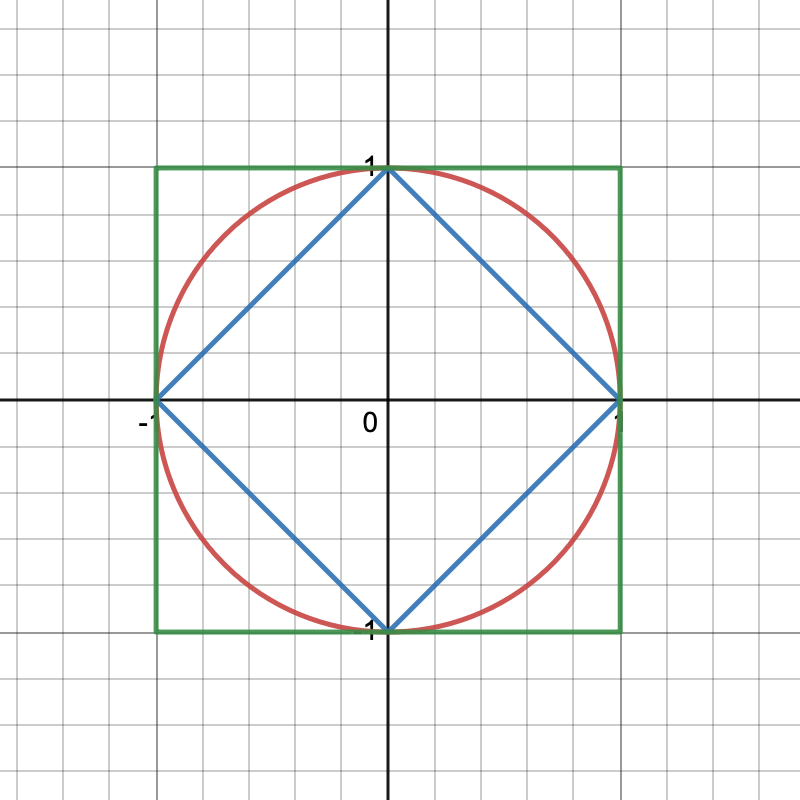
\includegraphics[width=0.5\textwidth,height=\textheight]{unitcircle.png}

We can even look at defining distances on other sets. For example, consider the set \(X = C^{0}([a,b])\), which is the set of all continuous functions \(f:[a,b] \to \mathbb{R}.\)\footnote{For the time being, think of these functions as ones that you can draw without lifting your pen off the page.} One way we can define the distance between two functions \(f\) and \(g\) is to consider evaluating them at all members of the domain, and finding what the maximum deviation between the two are. This gives rise to a metric \(d:X\times X \to \mathbb{R},\) namely \[d(f,g) := \max_{x \in [a,b]} \lvert f(x) - g(x) \rvert.\] Have a go at proving that this is a metric!

\hypertarget{convergence}{%
\subsubsection{Convergence}\label{convergence}}

In a similar way, have you noticed that the definitions of convergence for a real/complex sequence are pretty much identical? Again, this is because we can generalise the definition of convergence to metric spaces!

\BeginKnitrBlock{definition}[Convergence]
{\label{def:def4} }Let \((X,d)\) be a metric space, let \(a \in X\) and let \((a_n)_{n\in\mathbb{N}}\) be a sequence in \(X\). Then \((a_n)_{n\in\mathbb{N}}\) converges to \(a\) if \[\forall \epsilon > 0, \; \exists N = N(\epsilon) \in \mathbb{N}, \; \text{such that} \; \forall n \geq N, \; d(a_n,a) < \epsilon.\]
\EndKnitrBlock{definition}

This is a huge generalisation of Definition \ref{def:def2}, and you'll meet it properly in Analysis 2A next year!

\hypertarget{hints}{%
\section{Hints}\label{hints}}

As per usual, here's where you'll find the problem sheet hints!

\begin{enumerate}
\def\labelenumi{\arabic{enumi}.}
\item
  Use the definition! Try and follow a similar format to what we did in tutorials. Make sure to write things logically, and ensure that you've satisfied each part of the definition.
\item
  Again, this is an exercise in using the definition of convergence.
\item
  Without loss of generality, assume that \(\lvert z_1 \rvert \geq \lvert z_2 \rvert.\) The advice here is that if you ever get stuck in Analysis, either add \(0\), or multiply by \(1\) in a clever way. Try and do one of these tricks to allow you to apply the triangle inequality.
\item
  \begin{enumerate}
  \def\labelenumii{\alph{enumii})}
  \tightlist
  \item
    This is an \emph{if and only if} statement, so there are two things to prove! Try and manipulate the definition of convergence for one side of the \(\Leftrightarrow\) statement to resemble the other.
  \item
    Recall what it means for a complex number to be in modulus-argument form.
  \item
    Definition again, and follow the hint on the sheet.
  \item
    I'll leave this to you! Think simple!
  \end{enumerate}
\item
  For a) and b), De Moivre's Theorem will come in handy! For c), when bounding, remember that if you make a denominator smaller, the whole fraction will get bigger.
\end{enumerate}

\end{document}
